\documentclass{beamer}

%% Use the UCLouvain latest theme
%% \usetheme{UCL2018}

%% Load Latex packages
\usepackage{amssymb}
\usepackage{color}
\usepackage{float}
\usepackage[T1]{fontenc}
\usepackage{graphicx}
\usepackage{hyperref}
\usepackage[utf8]{inputenc}
\usepackage{lmodern}
\usepackage{makecell}
\usepackage[authoryear, round]{natbib}
\usepackage{ragged2e}
\usepackage{tikz} %% For drawing arrows
\usepackage{wrapfig}
\usepackage{xmpincl}
\usepackage{xspace}

%% Colors
%% ------
% Color panel used throughout the poster
\definecolor{lgray}{rgb}{0.9179688,0.9179688,0.9179688} % #ebebeb
\definecolor{dgray}{rgb}{0.796875,0.796875,0.796875} % #cccccc
\definecolor{vdgray}{rgb}{0.3984375,0.3984375,0.3984375} % #666666
\definecolor{coral}{rgb}{0.9960938,0.4960938,0.3125000} % #ff7f50
\definecolor{blue}{rgb}{0.4218750,0.6484375,0.8007812} % #6ca6cd
\definecolor{green}{rgb}{0.6992188,0.7265625,0.5078125} % #b3ba82
\definecolor{yellow}{rgb}{0.9570312,0.8671875,0.6992188} % #f5deb3


%% Coding fonts
%% ------------
%% Font for R chunks
\usepackage{listings}
\lstset{
  language=R,
  basicstyle=\footnotesize\ttfamily\color{vdgray}, % the size of the fonts that are used for the code
  numbers=left,                   % where to put the line-numbers
  numberstyle=\tiny\color{gray},  % the style that is used for the line-numbers
  stepnumber=1,                   % the step between two line-numbers.
  numbersep=0.1cm,                % how far the line-numbers are from the code
  backgroundcolor=\color{lgray},  % choose the background color. You must add \usepackage{color}
  deletekeywords={stat, model, matrix},
  keywordstyle=\color{blue},      % keyword style
  stringstyle=\color{green},      % string literal style
  xleftmargin=0.5cm,
}


%% Custom functions
%% ------------
%% Inline code highlight
\newcommand{\hcode}[2][lgray]{{\ttfamily\color{vdgray}\colorbox{#1}{#2}}}
%% Header that includes slide title + section title
\newcommand{\frametitlesection}[1]{\frametitle{\centering #1 \footnotesize \hspace{0pt plus 1 filll} \insertsection}}

%% Presentation metadata
%% ------------
\title{Standardised and reproducible analysis of mass spectrometry-based
single-cell proteomics data}
\subtitle{Replication of the SCoPE2 analysis by Specht et al. 2019}
% \subtitle{Slides available at: \url{}}
\author[]{Christophe Vanderaa, Laurent Gatto}
\date{18 August 2020}
\institute[]{Computational Biology Unit (CBIO), de Duve Institute, UCLouvain}

\begin{document}

\pdfinfo {/Author(Laurent Gatto - UCLouvain)}

%-----------------------------------------------
% Abstract
%-----------------------------------------------

%% Abstract: Recent advances in sample preparation, processing and mass
%% spectrometry (MS) have allowed the emergence of MS-based single-cell
%% proteomics (SCP). We present a robust and standardized workflow to reproduce
%% the data analysis of SCoPE2, one of the pioneering works in the field
%% developed by the Slavov Lab. The implementation uses well-defined
%% Bioconductor classes that provide powerful tools for single-cell RNA
%% sequencing and for MS-based proteomics. We demonstrate that our pipeline can
%% reproduce the SCoPE2 analysis using only a few lines of code.

% Apply the 'remember picture' style to all pictures that defines or uses
% external nodes
\tikzstyle{every picture}+=[remember picture]

%-----------------------------------------------
% Title page
%-----------------------------------------------

\begin{frame}[plain]
\titlepage
\end{frame}

%-----------------------------------------------
% Table of content
%-----------------------------------------------


\AtBeginSection[]{
  \setbeamercolor{section in toc}{fg=black}
  \setbeamerfont{section in toc}{size=\large}

  \mode<handout>{
    \setbeamercolor{background canvas}{bg=white}
    \setbeamercolor{section in toc}{fg=black}
  }

  \begin{frame}[plain]
    \frametitle{Outline}
    \tableofcontents[currentsection,hideothersubsections]
  \end{frame}

  \setbeamercolor{background canvas}{bg=white}
}


%-----------------------------------------------
% Introduction
%-----------------------------------------------

\section{Introduction}

\begin{frame}
  \frametitlesection{The value of replication (1)}

  \begin{itemize}
  \item<+-> Expectation
    
\includegraphics[width=\linewidth]{figs/expectation.png}
  \item<+-> Reality
    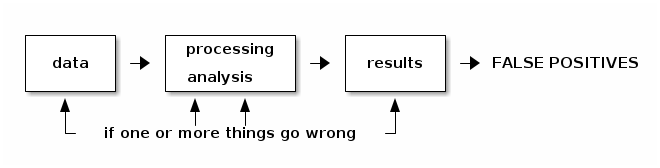
\includegraphics[width=\linewidth]{figs/reality.png}
  \end{itemize}
  
\end{frame}

\begin{frame}
  \frametitlesection{The value of replication (2)}

  \begin{itemize}
  \item \textbf{Reproduction-based development} agreement between the
    developer, the data producer and the user.
  \end{itemize}


  \bigskip
  
  Replication is the first step to define sound data infrastructure
  and principled analysis.
  
\end{frame}

\begin{frame}
  \frametitlesection{Why SCoPE2}
    \begin{itemize}
        \item{SCoPE2 quantifies thousands of proteins x thousands single-cells}
        \item{Full protocole available}
        \item{Full analysis script and data available}
    \end{itemize}


\end{frame}

\begin{frame}
    \frametitlesection{Our objectives}
  
    \begin{itemize}
    \item Contribute a standardized and principled data and analysis
      that is broadly applicable.

    \item Reproducible computational infrastructure to further
      improve data analysis and interpretation.

    \item  R/Bioconductor is an ideal environment to attain these goals.
      
    \end{itemize}

    \bigskip
    
    Implemented in the \hcode{scp} package.

\end{frame}


%-----------------------------------------------
% scp package
%-----------------------------------------------

\section{scp package}

\begin{frame}
    \frametitlesection{Data infrastructure: QFeatures\footnote{\citet{QFeatures}}}

    \centering
    \begin{columns}
        \begin{column}{0.8\textwidth}
            \hcode{QFeatures}: data framework dedicated to manipulate and process
            MS-based quantitative data.
        \end{column}
        \begin{column}{0.2\textwidth}
            
\includegraphics[width=\linewidth]{figs/sticker_QFeatures.png}
        \end{column}

    \end{columns}

    \bigskip

    \begin{tikzpicture}
    \node<1> (img1) {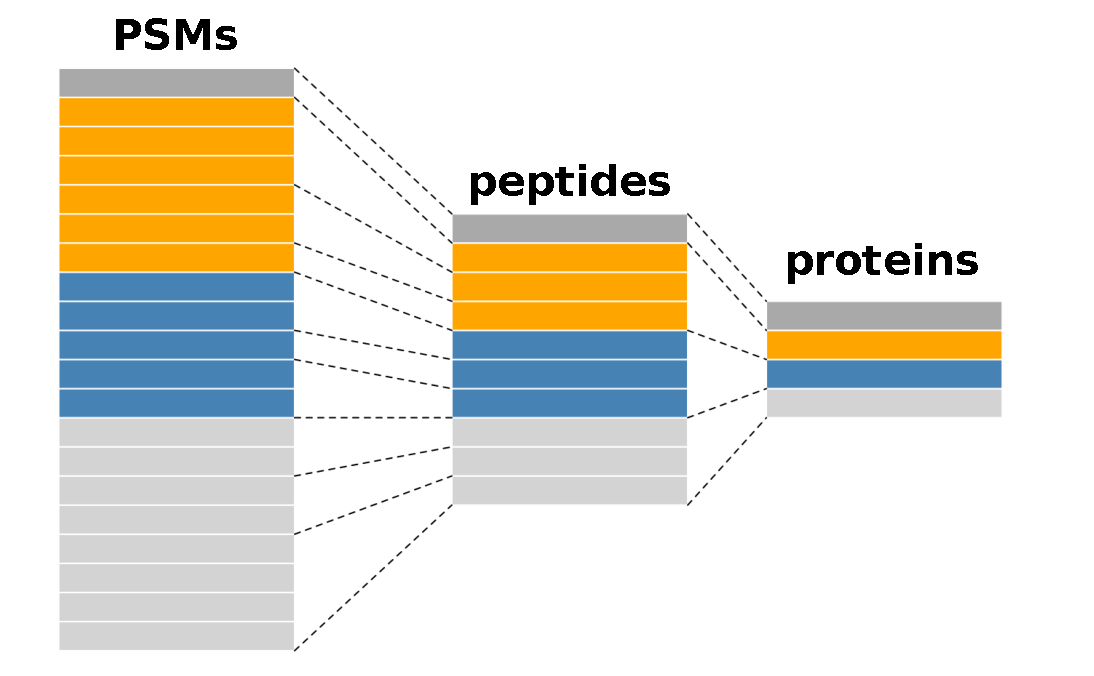
\includegraphics[width=0.8\linewidth]{figs/QFeatures.pdf}};
    \node<2> (img2) {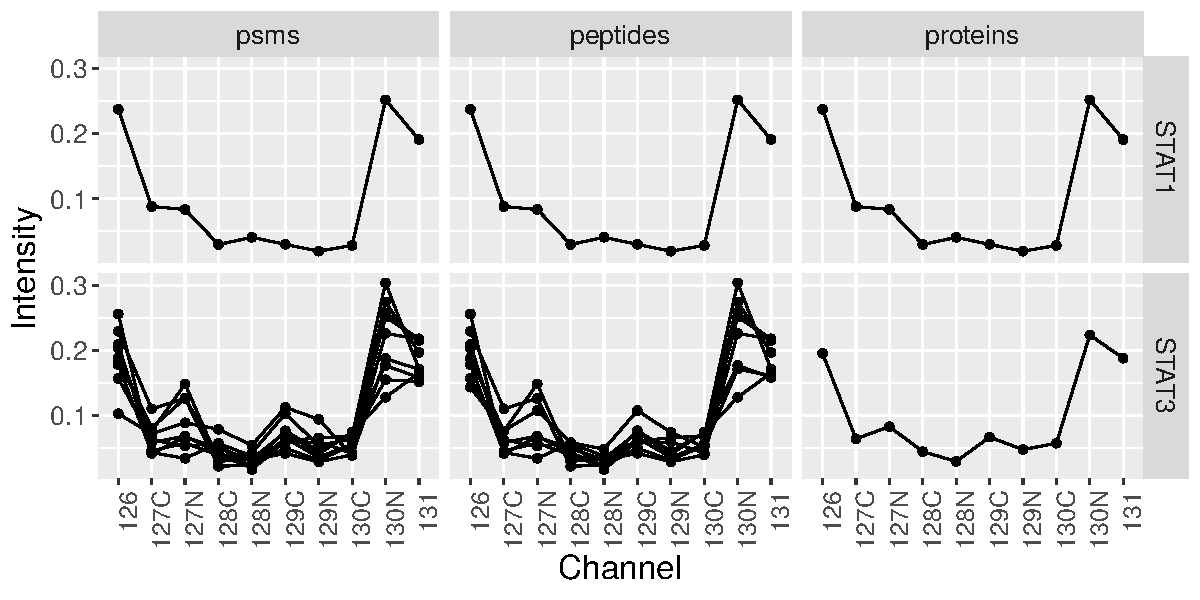
\includegraphics[width=0.8\linewidth]{figs/QFeatures_data.pdf}};
  \end{tikzpicture}

\end{frame}



\begin{frame}
    \frametitlesection{Data infrastructure: SingleCellExperiment\footnote{\citet{sce}}$^,$\footnote{\citet{Amezquita2019-bf}}}
    \begin{columns}
        \begin{column}{0.8\textwidth}
            \hcode{SingleCellExperiment}: provides dedicated framework for
            single-cell data analysis.
        \end{column}
        \begin{column}{0.2\textwidth}
            
\includegraphics[width=\linewidth]{figs/sticker_SingleCellExperiment.png}
        \end{column}
    \end{columns}

    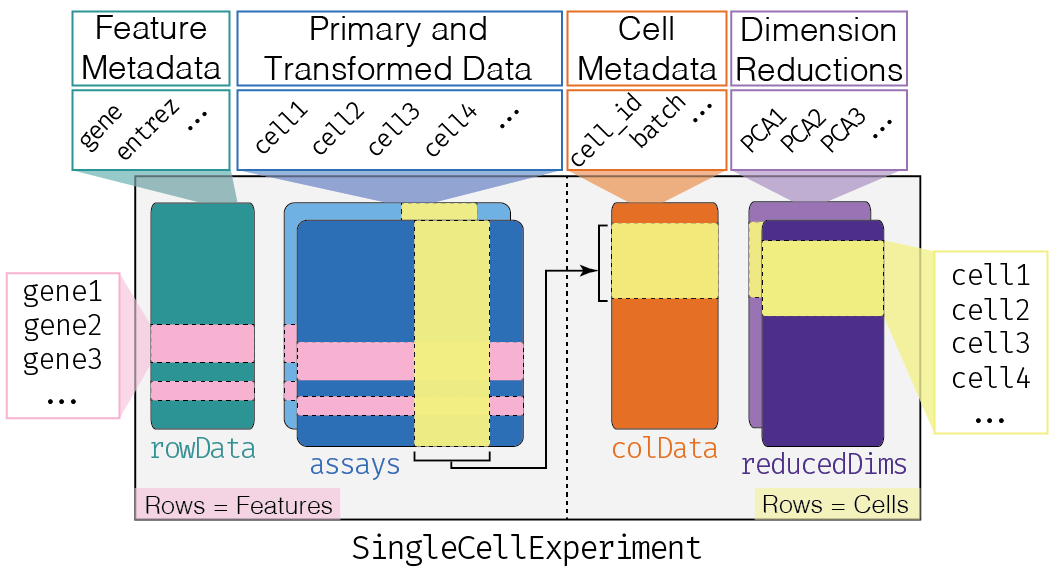
\includegraphics[width=0.9\linewidth]{figs/SingleCellExperiment.png}

\end{frame}


\begin{frame}
    \frametitlesection{Data infrastructure: scp}

    \hcode{scp} = \hcode{SingleCellExperiment} + \hcode{QFeatures}
    \begin{figure}
        \centering
        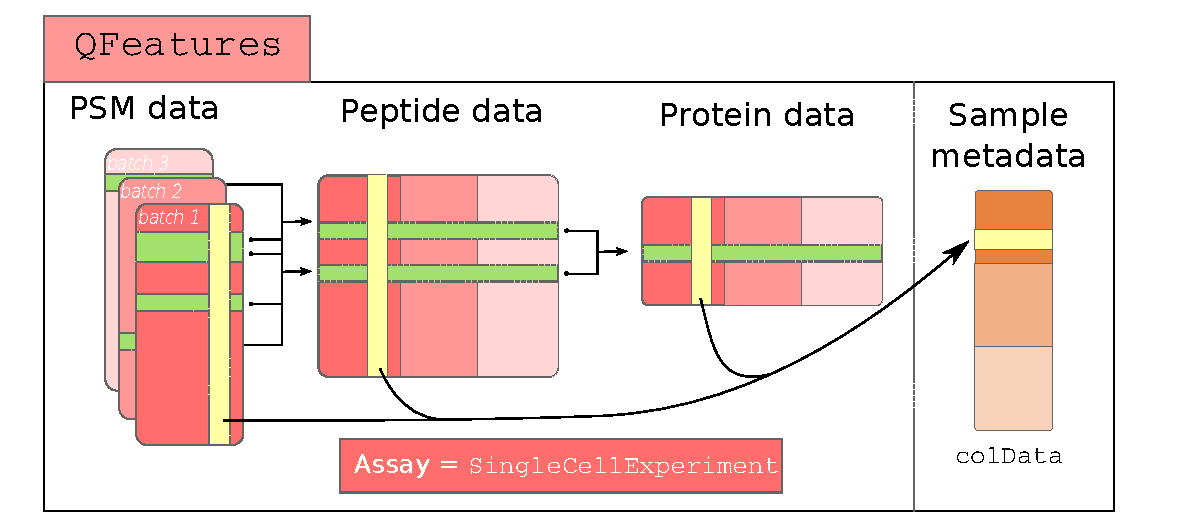
\includegraphics[width=\linewidth]{figs/SCP_framework.pdf}
    \end{figure}


\end{frame}

\begin{frame}[fragile]
    \frametitlesection{Load data}

    Load the SCoPE2 dataset called \hcode{specht2019v2}\footnote{\citet{Specht2019-jm}}

    \begin{lstlisting}
library(scpdata)
data("specht2019v2")
    \end{lstlisting}

    Dataset overview

    \begin{lstlisting}
show(specht2019v2)
    \end{lstlisting}

    \begin{lstlisting}[language = TeX, numbers = none, basicstyle = \tiny\ttfamily\color{vdgray}]
An instance of class QFeatures containing 179 assays:
 [1] 190222S_LCA9_X_FP94AA: SingleCellExperiment with 2823 rows and 11 col...
 [2] 190222S_LCA9_X_FP94AB: SingleCellExperiment with 4297 rows and 11 col...
 [3] 190222S_LCA9_X_FP94AC: SingleCellExperiment with 4956 rows and 11 col...
 ...
 [177] 191110S_LCB7_X_APNOV16plex2_Set_9: SingleCellExperiment with 4626 r...
 [178] peptides: SingleCellExperiment with 9208 rows and 1018 columns
 [179] proteins: SingleCellExperiment with 2772 rows and 1018 columns
    \end{lstlisting}

    \bigskip
    \footnotesize

    Tabular data (such as generated from MaxQuant, ProteomeDiscoverer,
    ...) can be read using the \hcode{readSCP()} function.

\end{frame}


\begin{frame}[fragile]
    \frametitlesection{Metadata}

    \hcode{colData} stores sample metadata for \textbf{all assays} in one table

    \begin{table}[!htbp]
        \makebox[\textwidth]{ % For centering because table is too large
        \centering
        \scriptsize
        \noindent
        \begin{tabular}{@{\extracolsep{5pt}} cccccc}
\\[-1.8ex]\hline
\hline \\[-1.8ex]
Set & Channel & SampleType & lcbatch & sortday & digest \\
\hline \\[-1.8ex]
190222S\_LCA9\_X\_FP94AA & RI1 & Carrier & LCA9 & s8 & N \\
190222S\_LCA9\_X\_FP94AA & RI2 & Reference & LCA9 & s8 & N \\
190222S\_LCA9\_X\_FP94AA & RI3 & Unused & LCA9 & s8 & N \\
190222S\_LCA9\_X\_FP94AA & RI4 & Macrophage & LCA9 & s8 & N \\
190222S\_LCA9\_X\_FP94AA & RI5 & Macrophage & LCA9 & s8 & N \\
190222S\_LCA9\_X\_FP94AA & RI6 & Macrophage & LCA9 & s8 & N \\
... & ... & ... & ... & ... & ... \\
\hline \\[-1.8ex]
        \end{tabular}
        }
    \end{table}
\end{frame}

\begin{frame}[fragile]
    \frametitlesection{Analysis workflow}

    \scriptsize

    \begin{enumerate}
        \item Load data
    \end{enumerate}

    \textbf{PSM data}

    \begin{lstlisting}[language = TeX, numbers = none, basicstyle = \ttfamily\@setfontsize{\srcsize}{5pt}{5pt}\color{vdgray}]
 [1] 190222S_LCA9_X_FP94AA: SingleCellExperiment with 2823 rows and 11 columns
 [2] 190222S_LCA9_X_FP94AB: SingleCellExperiment with 4297 rows and 11 columns
 [3] 190222S_LCA9_X_FP94AC: SingleCellExperiment with 4956 rows and 11 columns
 ...
 [177] 191110S_LCB7_X_APNOV16plex2_Set_9: SingleCellExperiment with 4626 rows and 16 columns
    \end{lstlisting}

    \pause

    \begin{enumerate}
        \setcounter{enumi}{1}
        \item \textbf<4>{PSM filtering}
        \item Expression channel by reference channel division
        \item PSM to peptides aggregating
        \item \textbf<4>{Single cells filtering based on median CV}
        \item Normalization
        \item \textbf<4>{Removal of highly missing peptides}
        \item \textbf<4>{Log-transformation}
    \end{enumerate}

    \textbf{Peptide data}

    \begin{lstlisting}[language = TeX, numbers = none, basicstyle = \ttfamily\@setfontsize{\srcsize}{5pt}{5pt}\color{vdgray}]
 [178] peptides: SingleCellExperiment with 9208 rows and 1018 columns
    \end{lstlisting}

    \pause

    \begin{enumerate}
        \setcounter{enumi}{8}
        \item \textbf<4>{Peptides to proteins aggregation}
        \item Normalization
        \item Imputation
        \item \textbf<4>{Batch correction}
    \end{enumerate}

    \textbf{Peptide data}

    \begin{lstlisting}[language = TeX, numbers = none, basicstyle = \ttfamily\@setfontsize{\srcsize}{5pt}{5pt}\color{vdgray}]
 [179] proteins: SingleCellExperiment with 2772 rows and 1018 columns
    \end{lstlisting}


\end{frame}

%-----------------------------------------------
% scp showcase
%-----------------------------------------------

\section{scp showcase}

\begin{frame}[fragile]
    \frametitlesection{PSM filtering}

    Filter out features based on the feature metadata

    \bigskip

    Example: filter out reverse hits. The filter is applied to the
    \hcode{Reverse} field in the feature metadata

    \begin{lstlisting}
filterFeatures(specht2019v2,
               ~ Reverse != "+")
    \end{lstlisting}

    Source code in \hcode{QFeatures}
\end{frame}

\begin{frame}[fragile]
    \frametitlesection{QC metrics (1)}
    \small
    Interesting metrics for MS-SCP quality control:

    \begin{itemize}
        \item{Sample to carrier ratio}: ratio of the carrier channel intensity
        signal over the sample channel intensity
        \item{Peptide FDR\footnote{false discovery rate}: expected rate of
        wrongly assigned features to a given peptide}
        \item{Cell median CV\footnote{coefficient of variation}: reliability of
        the protein quantification summarized over each cell.}
    \end{itemize}

    Example:

    \begin{lstlisting}
computeMedianCV(specht2019v2,
                i = "peptides",
                proteinCol = "protein",
                peptideCol = "peptide",
                batchCol = "Set")
    \end{lstlisting}

    Source code in \hcode{scp}

\end{frame}


\begin{frame}[fragile]
    \frametitlesection{QC metrics (2)}

    QC metrics are stored in the data set for plotting or subsetting

    \begin{lstlisting}[basicstyle = \scriptsize\ttfamily\color{vdgray}]
library(tidyverse)
specht2019v2[["peptides"]] %>%
  colData %>%
  data.frame %>%
  ggplot(aes(x = MedianCV,
             fill = SampleType)) +
  geom_histogram() +
  geom_vline(xintercept = 0.4)
    \end{lstlisting}

    \begin{figure}
        \centering
        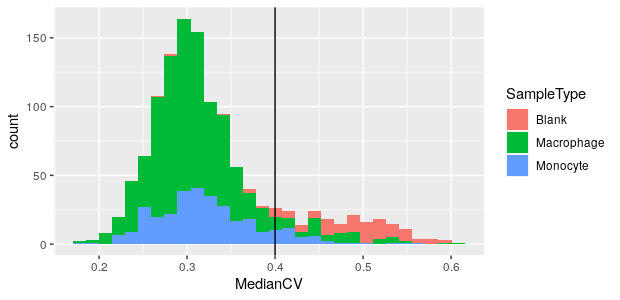
\includegraphics[width=.7\linewidth]{figs/medianCV.png}
    \end{figure}
\end{frame}

\begin{frame}[fragile]
    \frametitlesection{Feature aggregation}

    \begin{columns}
        \begin{column}{0.6\textwidth}
            Feature aggregation includes 2 steps:
            \begin{itemize}
                \item{Combine the quantiative data from multiple features to a
                single aggregated features}
                \item{Store the relationship between the parent features and the
                aggregated features}
            \end{itemize}
        \end{column}
        \begin{column}{0.4\textwidth}
            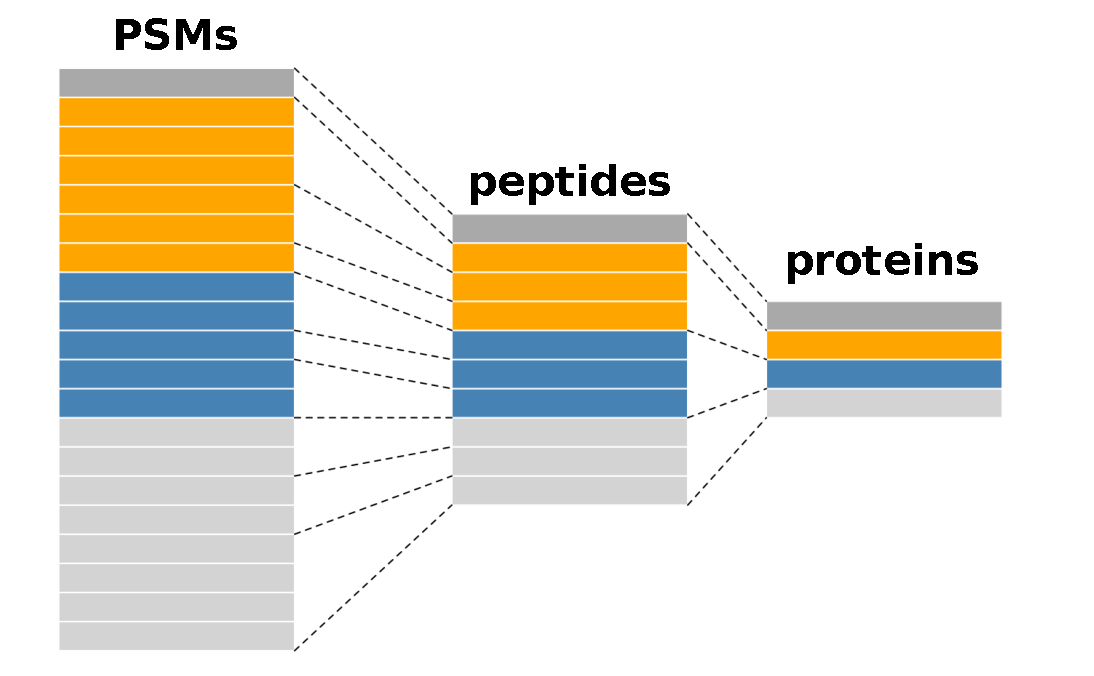
\includegraphics[width=\textwidth]{figs/QFeatures.pdf}
        \end{column}
    \end{columns}

    \bigskip

    Example: aggregate peptides to proteins

    \begin{lstlisting}
aggregateFeatures(specht2019v2,
                  i = "peptides",
                  name = "proteins",
                  fcol = "protein",
                  fun = colMedians, na.rm = TRUE)
    \end{lstlisting}

    Source code in \hcode{QFeatures}

\end{frame}


\begin{frame}[fragile]
    \frametitlesection{Managing missingness}

    \hcode{0}'s can be either \textbf{biological} or \textbf{technical} zero.
    They are better relaced by \hcode{NA}'s.

    \begin{lstlisting}
zeroIsNA(specht2019v2,
         i = "peptides")
    \end{lstlisting}

    Features containing too many missing data (e.g. >= 99 \%) should be removed

    \begin{lstlisting}
filterNA(specht2019v2,
         i = "peptides",
         pNA = 0.99)
    \end{lstlisting}

    Source code in \hcode{QFeatures}

\end{frame}

\begin{frame}[fragile]
    \frametitlesection{Data transformation}

    Common data transformation can easily be applied:

    \begin{itemize}
        \item{Normalization}
        \item{Log-transformation}
        \item{Imputation}
    \end{itemize}

    Example: $log_2$-transformation:

    \begin{lstlisting}
logTransform(specht2019v2,
             i = "peptides",
             base = 2,
             name = "peptides_log")
    \end{lstlisting}

    Source code in \hcode{QFeatures}

\end{frame}

\begin{frame}[fragile]
    \frametitlesection{Custom functions}

    Some custom function can be applied to the data set too.

    Example: batch correction using \hcode{sva::ComBat}. First, extract the data

    \begin{lstlisting}[basicstyle = \scriptsize\ttfamily\color{vdgray}]
sce <- specht2019v2[["proteins"]]
    \end{lstlisting}

    Build the correction matrix and apply the ComBat algorithm

    \begin{lstlisting}[basicstyle = \scriptsize\ttfamily\color{vdgray}]
batch <- colData(sce)$Set
model <- model.matrix(~ SampleType, data = colData(sce))
assay(sce) <- ComBat(dat = assay(sce),
                     batch = batch,
                     mod = model)
    \end{lstlisting}

    Add the corrected protein to the dataset and keep feature relationships

    \begin{lstlisting}[basicstyle = \scriptsize\ttfamily\color{vdgray}]
addAssay(specht2019v2,
         sce,
         name = "proteins_batchC") %>%
addAssayLinkOneToOne(from = "proteins",
                     to = "proteins_batchC")
    \end{lstlisting}


\end{frame}

%-----------------------------------------------
% Replication results
%-----------------------------------------------

\section{Replication results}

\begin{frame}
    \frametitlesection{Selected features}

    \centering
    \textbf{Peptides} \\
    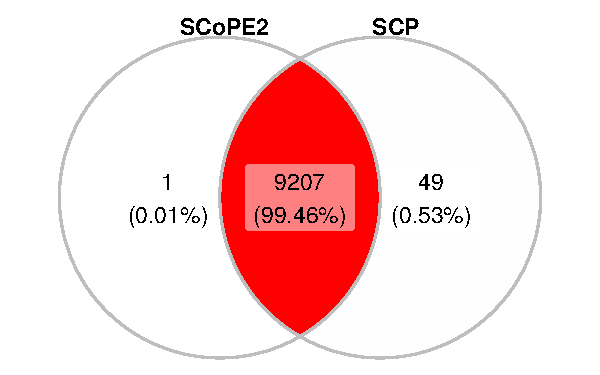
\includegraphics[width=0.5\textwidth]{figs/Benchmark_pep_venn.pdf} \\
    \textbf{Proteins}\\
    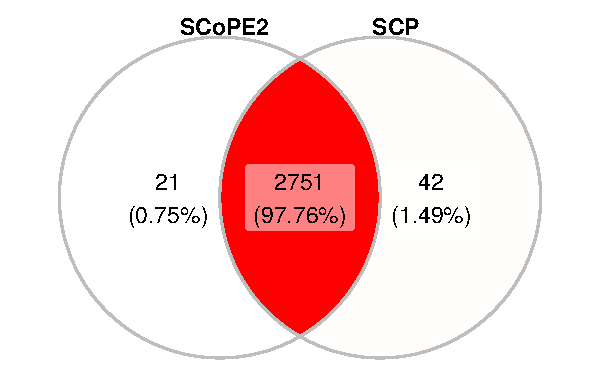
\includegraphics[width=0.5\textwidth]{figs/Benchmark_prot_venn.pdf}

\end{frame}

\begin{frame}
    \frametitlesection{Numerical comparison}

    \centering
    \textbf{Peptides} \\
    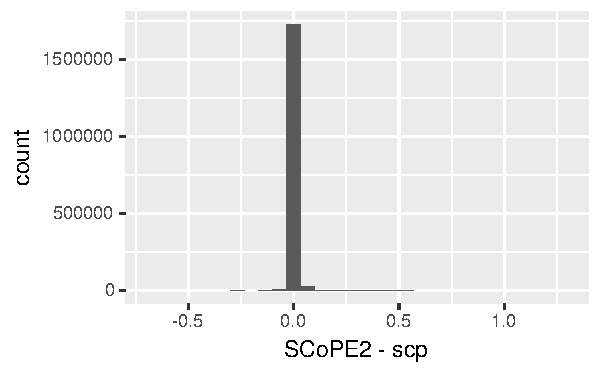
\includegraphics[width=0.5\textwidth]{figs/Benchmark_pep_err.pdf} \\
    \textbf{Proteins}\\
    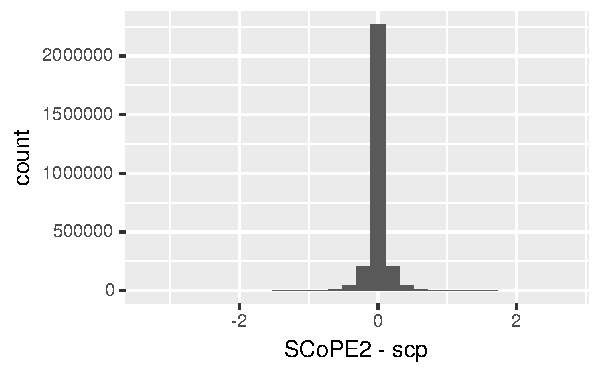
\includegraphics[width=0.5\textwidth]{figs/Benchmark_prot_err.pdf}

\end{frame}


\begin{frame}
    \frametitlesection{Replicate weighted PCA}

    \begin{columns}
        \begin{column}{0.5\textwidth}
            \textbf{SCoPE2}
            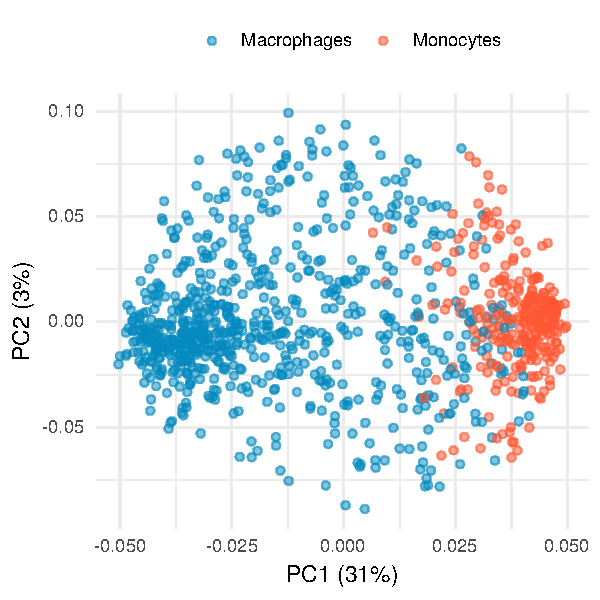
\includegraphics[width=\textwidth]{figs/wPCA_SCoPE2.pdf}
        \end{column}
        \begin{column}{0.5\textwidth}
            \textbf{scp}
            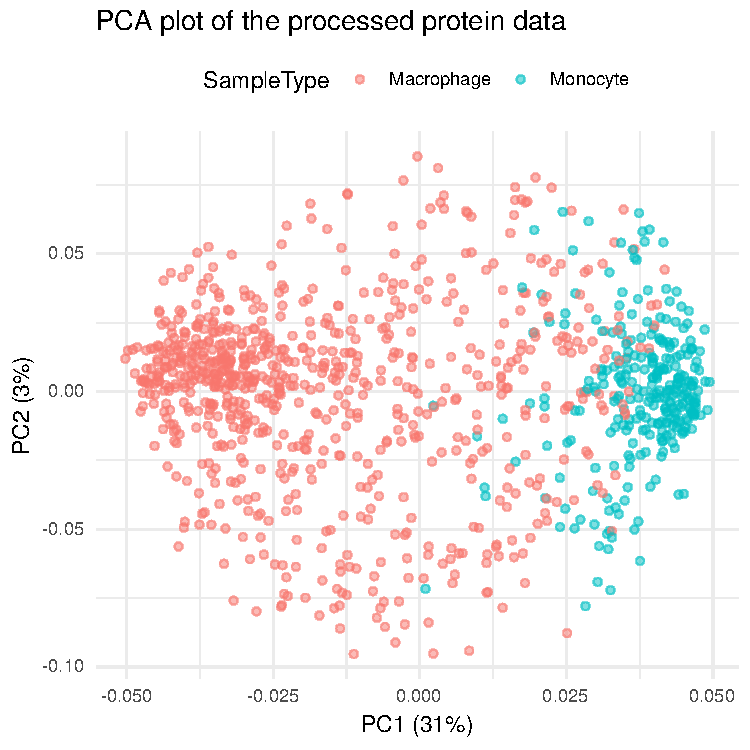
\includegraphics[width=\textwidth]{figs/wPCA_scp.pdf}
        \end{column}
    \end{columns}
\end{frame}

\begin{frame}
    \frametitlesection{Note about replication }

    \textbf{Versioning} is essential for replication

    Example: batch correction using the \hcode{ComBat} algorithm from \hcode{sva}

    \bigskip

    \scriptsize
    \centering
    \begin{columns}
        \begin{column}{0.5\textwidth}
            \hcode{sva 3.34.0}
            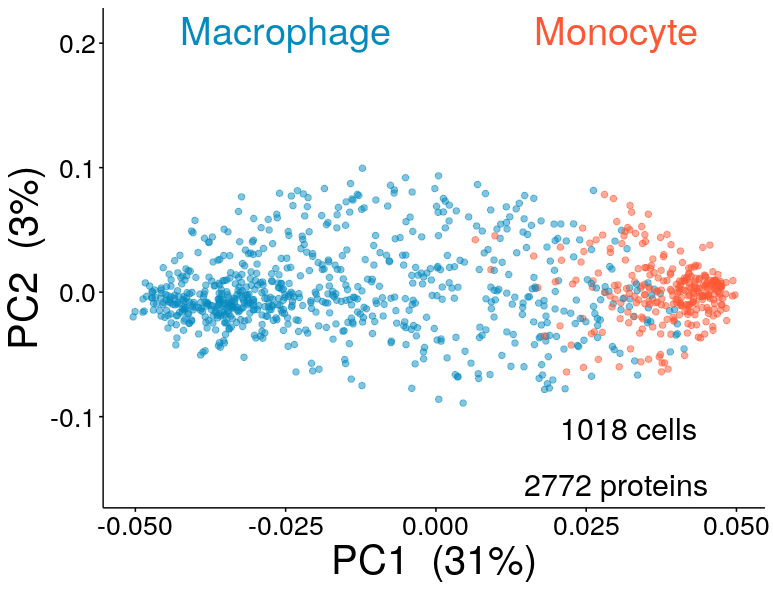
\includegraphics[width=\textwidth]{figs/CombatOld.png}
        \end{column}
        \begin{column}{0.5\textwidth}
            \hcode{sva 3.36.0}
            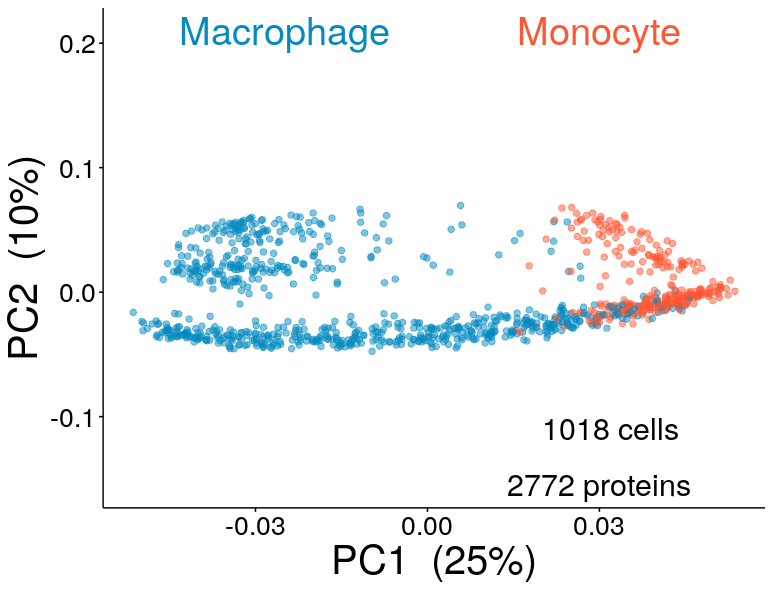
\includegraphics[width=\textwidth]{figs/CombatNew.png}
        \end{column}
    \end{columns}

\end{frame}


%-----------------------------------------------
% Conclusion
%-----------------------------------------------

\section{Conclusion}


\begin{frame}
  \frametitlesection{Take home message}  
  \begin{itemize}
  \item MS-based single cell proteomics: young field, with many
    challenges and great progess. \hcode{scp} to address the need for
    principled and reproducible data analysis.
  \item \hcode{scp} isn't specific to SCoPE2/TMT data, applicable to
    other LF protocols such as nanoPOTS (\citet{Williams2020-nv,Cong2020-kh}).
  \item \hcode{scp} and \hcode{SingleCellExperiment}: same
    infrastructure for single cell proteomics and RNA sequencing.
  \item Tool for novel computational developments.
    
  \end{itemize}
\end{frame}

\begin{frame}
  %% modelling
    \frametitlesection{Future directions}
    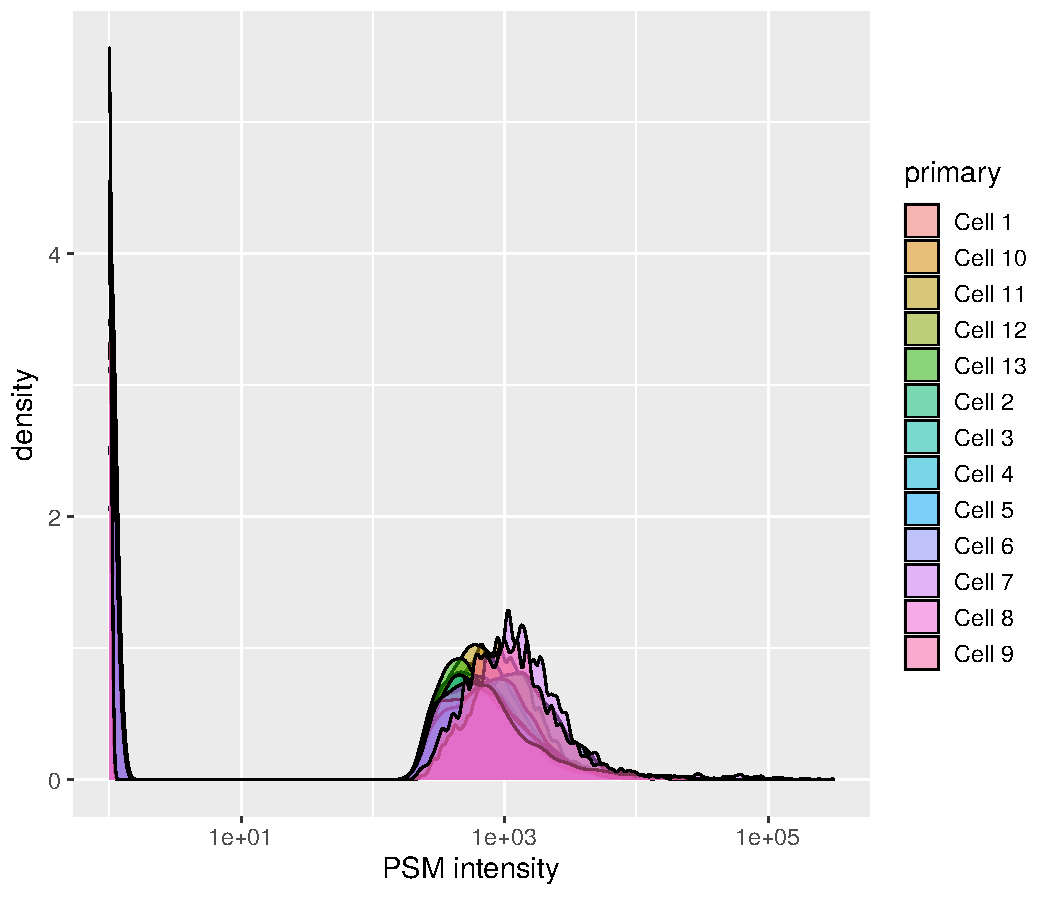
\includegraphics[width=.5\linewidth]{figs/PSM_intensity.pdf}
    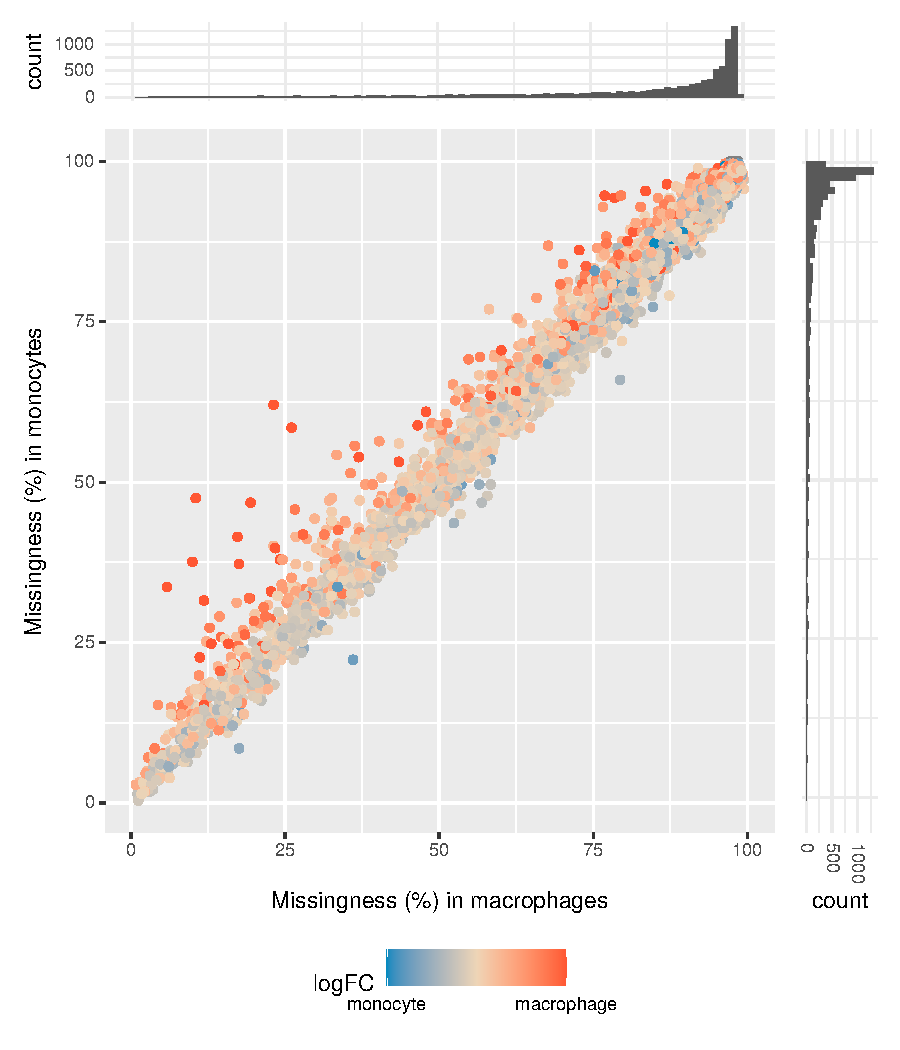
\includegraphics[width=.4\linewidth]{figs/missingness.pdf}

\end{frame}


\begin{frame}
    \frametitlesection{Resources}

    \textbf{Packages}

    \begin{itemize}
        \item \hcode{scp}: \url{http://UClouvain-CBIO.github.io/scp}
        \item \hcode{scpdata}: coming soon
        \item \hcode{QFeatures}: \url{http://rformassspectrometry.github.io/QFeatures}
        \item \hcode{SingleCellExperiment}: Bioconductor
    \end{itemize}


    \bigskip

    \textbf{Slides}: \url{http://bit.ly/2020SCP} under CC-BY SA

\end{frame}

\begin{frame}
    \frametitlesection{Acknowledgements}

    \begin{itemize}
    \item Nikolai Slavov, Harrison Specht, Ed Emmott.
    \item Fonds National de la Recherche Scientifique (FNRS)
    \end{itemize}

    \bigskip

    \textbf{Thank you for your attention}
    
    
\end{frame}



%-----------------------------------------------
% References
%-----------------------------------------------

\begin{frame}[allowframebreaks]{References}
  \scriptsize
  \bibliographystyle{plainnat}
  \bibliography{ref}
\end{frame}



\end{document}
